%% BREAK LINES EVERY 80 CHARACTERS TO HELP GIT WITH MERGING
\subsection{Program Entry and Preprocessing}
The program entry point is in |main.py|; other local modules used in the 
algorithm are contained in the following directory structure.
\bgroup
\footnotesize
\itemsep=-1ex
\setlength{\columnsep}{-24pt}
\begin{multicols}{2}
\raggedbottom
\begin{itemize}[topsep=-12pt,leftmargin=22pt]
	\item[\file] |main.py|
	\item[\folder] |crossover/|
	\begin{itemize}[topsep=-1ex,leftmargin=12pt,itemsep=-.5ex]
		\item[\file] |__init__.py|
		\item[\file] |inver_over.py|
	\end{itemize}
	\item[\folder] |fitness/|
	\begin{itemize}[topsep=-1ex,leftmargin=12pt,itemsep=-.5ex]
		\item[\file] |__init__.py|
		\item[\file] |distance.py|
		\item[\file] |fitness.py|
	\end{itemize}
	\item[\folder] |ga_helper/|
	\begin{itemize}[topsep=-1ex,leftmargin=12pt,itemsep=-.5ex]
		\item[\file] |__init__.py|
		\item[\file] |offspring.py|
	\end{itemize}
	\item[\folder] |timing/|
	\begin{itemize}[topsep=-1ex,leftmargin=12pt,itemsep=-.5ex]
		\item[\file] |__init__.py|
	\end{itemize}
	\vfill\null
	\columnbreak
	\item[\folder] |mutation/|
	\begin{itemize}[topsep=-1ex,leftmargin=12pt,itemsep=-.5ex]
		\item[\file] |__init__.py|
		\item[\file] |scramble.py|
		\item[\file] |swap.py|
	\end{itemize}
	\item[\folder] |population/|
	\begin{itemize}[topsep=-1ex,leftmargin=12pt,itemsep=-.5ex]
		\item[\file] |__init__.py|
		\item[\file] |candidates.py|
		\item[\file] |initialization.py|
	\end{itemize}
	\item[\folder] |selection/|
	\begin{itemize}[topsep=-1ex,leftmargin=12pt,itemsep=-.5ex]
		\item[\file] |__init__.py|
		\item[\file] |parent.py|
		\item[\file] |survival.py|
	\end{itemize}
\end{itemize}
\end{multicols}
\egroup

Initialization is done in |main.py| through a call to |initialization.init_file()| in 
the |population| module, which takes a path to a file and returns a 
|numpy.ndarray| object containing the $x$- and $y$-coordinate pairs of the 
cities in the data file.

{\small\lstinputlisting[style=pycode]{include/snippets/init_file.py}}

The array returned from this function is then passed to the |Distances()| 
class constructor in the |fitness.distance| module and the |gen_all()| 
method is called on this object to generate all $\frac{1}{2}(n^2-n)$
distances.

{\small\lstinputlisting[style=pycode]{include/snippets/gen_all.py}}

The |_weighted_adjacency| instance variable of the object is then passed 
to the main function; this way |main()| can run multiple times without reloading 
and recomputing the same data.

\subsection{GA Initialization}
Immediately in |main()|, variables such as generation limit $G$, candidate pool size $CP$, 
mating pool size $MP$, and so on are defined. 

Candidates are then chosen by choosing $CP$ enumerations from the set of 
permutations of $\{0, 1, \ldots, n-1\}$, where $n$ is the number of cities.
Following this part of the algorithm's initialization, the |adjacent_distance()| function
is invoked on for the population. This function calls |single_cand_adjacent_distance|,

{\small\lstinputlisting[style=pycode]{include/snippets/sing_dist.py}}

\noindent which uses the adjacency matrix constructed in preprocessing to form 
an array of pairwise distances between each adjacent set of cities in the 
individual. Note that |end_idx| is defined as |city_idx[(i+1) % city_idx.shape[0]]|,
\ie the index of |city_idx| being accessed is found modulo 
|city_idx.shape[0]|${} = n$ so this computes distance from the last city on the 
tour back to the first. From the returned sequences of distances, we 
compute overall fitness of each individual in the pool (using \eqref{eq:fit1}
with the optimization discussed in sub-section~\ref{ssec:cheap}).

\subsection{GA Operators}
Within a loop that iterates $G$ times, the first operation performed is parent
selection using the multi-pointer selection (MPS) operator. MPS randomly 
selects an individual from one of $MP$ evenly spaced segments from the 
candidate pool and adds it to the parent pool. The operator then chooses
$MP-1$ other individuals at regular intervals of $CP/MP$. MPS was primarily 
chosen to minimize the risk of elitist selection emerging in our 
algorithm (\ie selecting only the fittest candidates), which leads to a 
high chance of the algorithm peaking at a local minima extremely early.

Inver-over is then introduced as the crossover operator, which in addition 
to the mutation operators discussed below, alters the offspring of the parent candidates 
selected by MPS. This operation prevents
the GA from plateauing at a local minima while promoting the exploration 
aspect of the algorithm by inverting a random segment at the crossover phase, 
based on the individuals in the mating pool.

Initial implementations of the algorithm used scramble as a mutation operator
and $\mu + \lambda$ survival selection. Preliminary tests showed that the 
randomness introduced by the swap mutation could be harmful to a fit 
individual more often than it was beneficial.  

Instead, a system was developed that considers the previous two generations'
top fitnesses when deciding which operator(s) to use for the next generation.
This is done by comparing variables |current_best_fitness| and 
|previous_best_fitness|; if optimal generational fitness is not improving
then introduce more randomness, otherwise maintain moderate randomness.

Varied amounts of randomness were selected by adding swap mutation --- 
which simply swaps two cities on the tour, depicted in Figure~\ref{fig:swap} --- instead 
of just scramble.
\begin{figure}[h]
	\centering
	\begin{subfigure}{\linewidth}
		\centering 
		\fbox{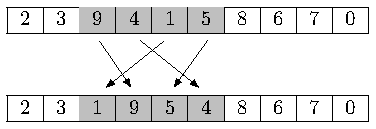
\includegraphics[width=0.9\linewidth]{include/graphs/mutation/scramble}}
		\caption{Scramble Mutation\label{fig:scramble}}
	\end{subfigure}
	\par\vskip12pt
	\begin{subfigure}{\linewidth}
		\centering 
		\fbox{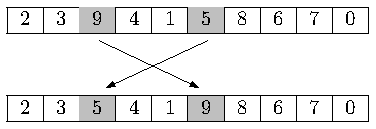
\includegraphics[width=0.9\linewidth]{include/graphs/mutation/swap}}
		\caption{Swap Mutation\label{fig:swap}}
	\end{subfigure}
	\caption{Two Types of Mutation Implemented}
\end{figure}
In such cases where generational fitness was not improving, 
scramble mutation (Figure~\ref{fig:scramble}) was favoured $4:1$, the mutation rate was increased, crossover
rate was decreased $1:2$, severity of mutation\footnote{See
sub-sub-section~\ref{sssec:severity}.}
was increased fourfold, and survivor selection was done favouring the 
replacement operator, rather than $\mu + \lambda$.  
Replacement was favoured $3:1$ here because the new (more random) individuals 
may initially score lower (\ie higher Hamiltonian cycle distance) than existing 
individuals, however their varied genetic make-up could allow them to escape 
local minima more effectively. Such a 
scenario with $\mu + \lambda$ would result in many or all of the newer, less 
fit individuals immediately being removed from the population. When generational
fitness is improving, the two mutation types are favoured evenly, mutation rate is 
lowered back to $10\%$, crossover rate is reset to $90\%$, and survival
selection favours $\mu + \lambda$ $75\%$ of the time.

\subsubsection{Severity in the Scramble Mutation}\label{sssec:severity}
As the scramble mutation is now being used when randomness is desirable, the 
decision to capitalize on this operator's strength was made. The implementation
of this involves a mutation factor $f_m \in (0, 1)$. 

{\small\lstinputlisting[style=pycode]{include/snippets/scramble.py}}
\noindent A mutation threshold is then defined by ${t_m := f_m \cdot n}$. 
Two indices, |start_idx| and |end_idx|, both between $0$ and $n-1$, are 
selected at random from the individual. If |end_idx|${}-{}$|start_idx|${}< t_m$
then the algorithm chooses new indices until this requirement is satisfied.

Consequently, when high entropy is required a mutation factor can be chosen 
to enforce this (\eg if $f_m = 0.4$ then no less than $40\%$ of the individual
will be scrambled).
